\documentclass{article}
\usepackage[utf8]{inputenc}
\usepackage{authblk}
\usepackage{setspace}
\usepackage[margin=1.25in]{geometry}
\usepackage{graphicx}
\usepackage{xcolor}
\usepackage{float}
\graphicspath{ {./figures/} }
\usepackage{amsmath,amssymb,amsfonts}
\usepackage{booktabs}
\usepackage{natbib}
\usepackage{hyperref}
\hypersetup{colorlinks=true, linkcolor=blue, citecolor=blue, urlcolor=blue}

\title{\textbf{Tariff-Related Executive Social Media Posts and Next-Day US Equity and Implied Volatility Reactions}}
\author[1]{SIQuant Research}
\affil[1]{Hypothesis $\times$ Quant}
\date{\today}
\onehalfspacing

\begin{document}
\maketitle

\begin{abstract}
\noindent \textbf{Hypothesis:} $H_0$: next-day S\&P 500 absolute abnormal return, signed abnormal return and VIX change after a tariff-related post equal those of ordinary days; $H_1$: they differ \\
\textbf{Data:} 428 Truth Social posts matching the keyword `tariff', 237 distinct reaction days among 1,117 sessions (2022-05-12 to 2026-10-23) \\
\textbf{Method:} Reaction window is the first session strictly after the post; baseline is the trailing 250-day mean; 5000-draw placebo over non-event days; Bonferroni $\alpha=0.0167$ \\
\textbf{Results:} abs return: event 0.736\% vs other 0.724\% (placebo $p=0.772$); signed return: event -0.023\% vs other 0.026\% (placebo $p=0.375$); vix change: event 0.810\% vs other 0.073\% (placebo $p=0.070$).
\end{abstract}

\section{Design}
Posts are selected by keyword only, so no text classifier can leak sentiment. Using the session after the post date guarantees that the measured reaction is not contaminated by the same-day move that may have prompted the post \citep{mackinlay1997event}. Event days are not independent when posts cluster; the placebo draws random days from the same sample rather than assuming normal errors.

\section{Results}
\begin{table}[h!]
\centering
\caption{Reaction on the first trading day after a tariff post}
\label{tab:event}
\begin{tabular}{lccc}
\toprule
Measure & Event days & Other days & Placebo $p$ \\
\midrule
$|$AR$|$ S\&P 500 (\%) & 0.736 & 0.724 & 0.7720 \\
AR S\&P 500 (\%) & -0.023 & 0.026 & 0.3747 \\
$\Delta$VIX (\%) & 0.810 & 0.073 & 0.0696 \\
\bottomrule
\end{tabular}
\end{table}


\begin{figure}[H]
\centering
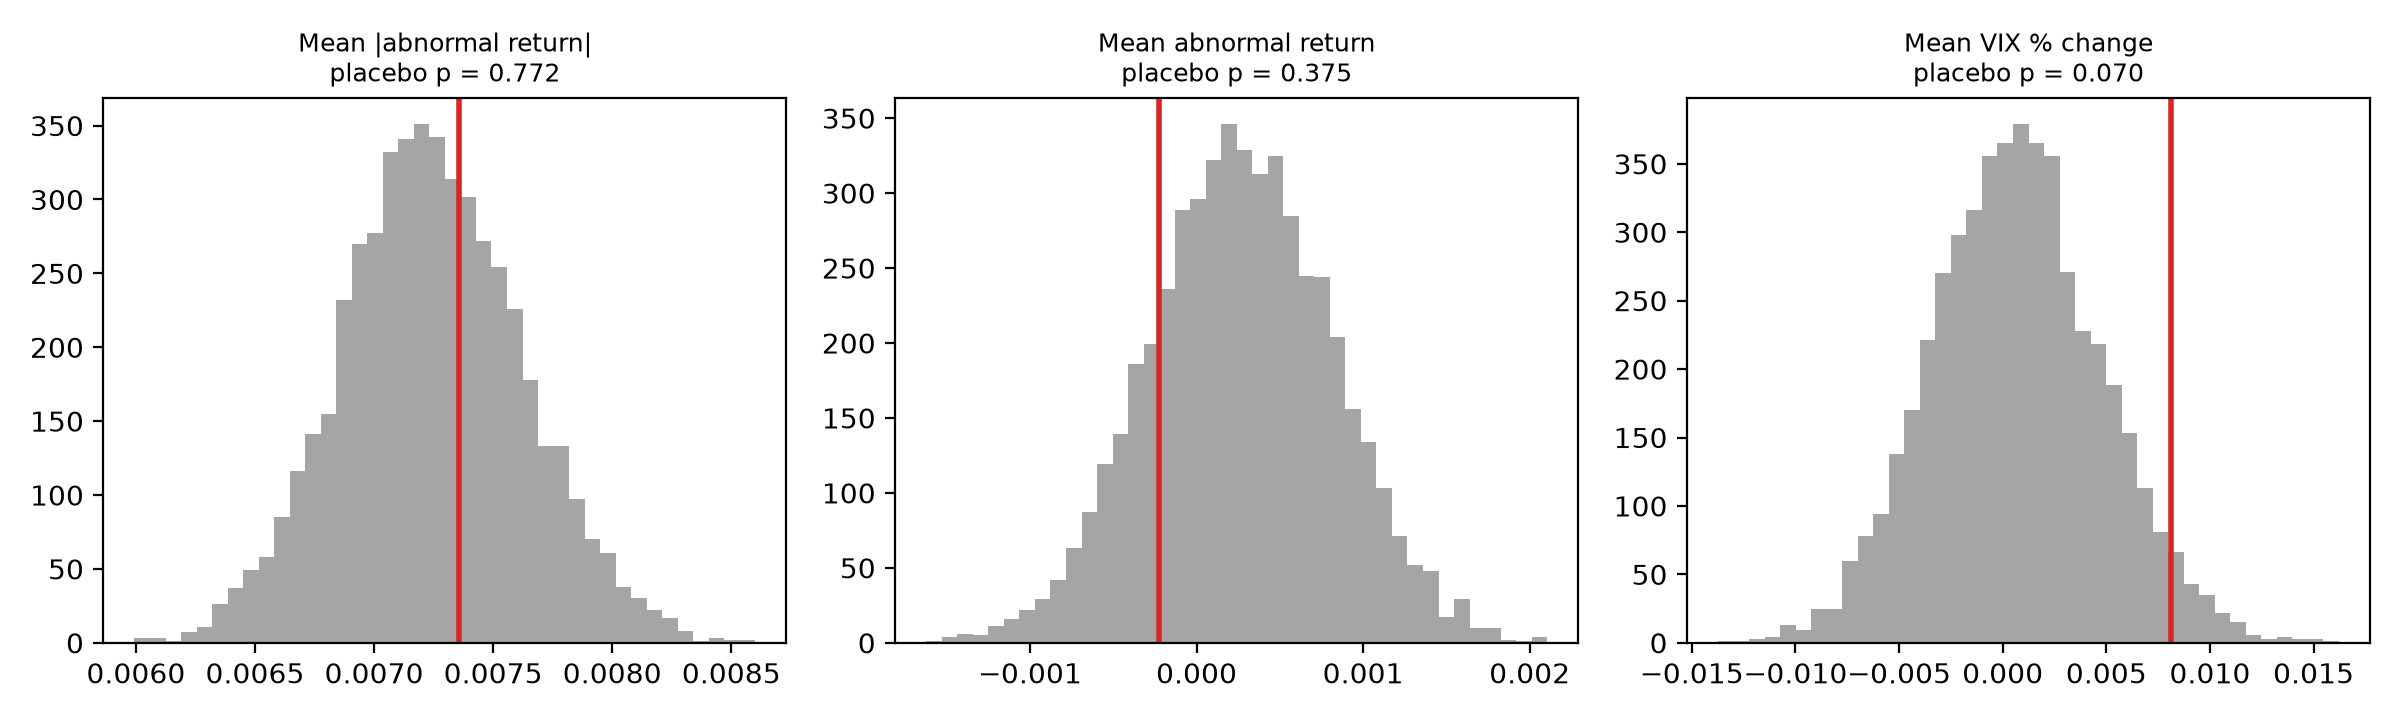
\includegraphics[width=\textwidth]{fig1_tariff_event_placebo.png}
\caption{Observed event-day mean (red) against the placebo distribution.}
\end{figure}

\section{Limitations}
Next-day windows discard the intraday reaction. Keyword matching ignores context. Truth Social coverage starts in 2022, so tariff episodes before that are missing.


\bibliographystyle{plainnat}
\bibliography{references}

\end{document}
